\maketitle
\tableofcontents
\newpage
\section{Theorie}
\section{Durchführung}
\subsection{Versuchsaufbau}
\subsection{Versuchsdurchführung}
\section{Auswertung}
\subsection{Bestimmung der Schallgeschwindigkeit in Acryl}
Die aus der Messung nach dem Impuls-Echo-Verfahren gewonnenen Messwerte finden sich
in Tabelle \ref{tab:1} , die aus dem Durchschallungsverfahren in Tabelle \ref{tab:2}.
\begin{figure}
  \centering
  \begin{subtable}{0.49\textwidth}
    \centering
    \begin{tabular}{c c c c}
      \toprule
      $l$/\si{\milli\metre} & $U$/\si{\volt} & $\symup{\Delta}t$/\si{\micro\second} & TGC/\si{\decibel} \\
      \midrule
      31 & 0.202 & 23.16 & 0 \\
      40.1 & 0.193 & 29.68 & 0 \\
      61.58 & 0.31 & 45.62 & 17.81 \\
      71.3 & - & 52.46 & 20.58 \\
      80.2 & 0.154 & 59.66 & 18.16 \\
      102 & 0.105 & 75.90 & 32.85 \\
      121.18 & 0.105 & 88.38 & 32.85 \\
      \bottomrule
    \end{tabular}
    \caption{Messwerte der Messung per Impuls-Echo-Verfahren. Bei den $\symup{\Delta}t$-
    Werten handelt es sich um die doppelte Laufzeit.}
    \label{tab:1}
  \end{subtable}
  \begin{subtable}{0.49\textwidth}
    \centering
    \begin{tabular}{c c c c}
      \toprule
      $l$/\si{\milli\metre} & $U$/\si{\volt} & $\symup{\Delta}t$/\si{\micro\second} & TGC/\si{\decibel} \\
      \midrule
      31 & 0.729 & 12.48 & 0 \\
      40.1 & 0.759 & 15.46 & 0 \\
      61.58 & 0.271 & 23.70 & 0 \\
      71.3 & - & 27.18 & 0 \\
      80.2 & 0.154 & 30.50 & 0 \\
      102 & 0.271 & 38.71 & 15.48 \\
      121.18 & 0.329 & 45.19 & 17.99 \\
      \bottomrule
    \end{tabular}
    \caption{Messwerte der Messung per Durchschallungsverfahren.}
    \label{tab:2}
  \end{subtable}
  \caption{$l$ bezeichnet jeweils die Höhe der Zylinder, $U$ die Spannungsamplitude des
  gemessenen Peaks, $\symup{\Delta}t$ den zeitlichen Abstand zwischen senden des Schallimpulses
  und empfangen des Signals und TGC gibt den verwendeten Verstärkungsfaktor für
  den Amplitudenwert an.}
\end{figure}
Die Bestimmung der Schallgeschwindigkeiten gescheiht nun durch lineare Regression.
Dies ist notwendig, da innerhalb des Sondenmaterials eine gewisse Strecke zurückgelegt werden
muss, die ansonsten als systematischer Fehler in die Rechnung eingehen würden.
Regression der Länge-Laufzeit Wertepaare mit
\begin{equation}
  t(l) = l \cdot \frac{1}{c} + t_0
\end{equation}
(wobei $c$ die Schallgeschwindigkeit im Zylinder und $t_0$ die Laufzeit innerhalb der
Sonde ist) liefert für das Impuls-Echo-Verfahren:
\begin{align*}
  c &= \SI[per-mode=reciprocal]{2740(24)}{\metre\per\second}\\
  t_0 &= \SI{0.28(25)}{\micro\second}
\end{align*}
und für das Durchschallungsverfahren:
\begin{align*}
  c &= \SI[per-mode=reciprocal]{2727(21)}{\metre\per\second}\\
  t_0 &= \SI{1.0(2)}{\micro\second}
\end{align*}
Messwerte und Regression sind in Abbildung \ref{abb:1} für das Impuls-Echo-Verfahren,
sowie in Abbildung \ref{abb:2} für das Durchschallverfahren dargestellt.
\begin{figure}
  \centering
  \begin{subfigure}{0.49\textwidth}
    \centering
    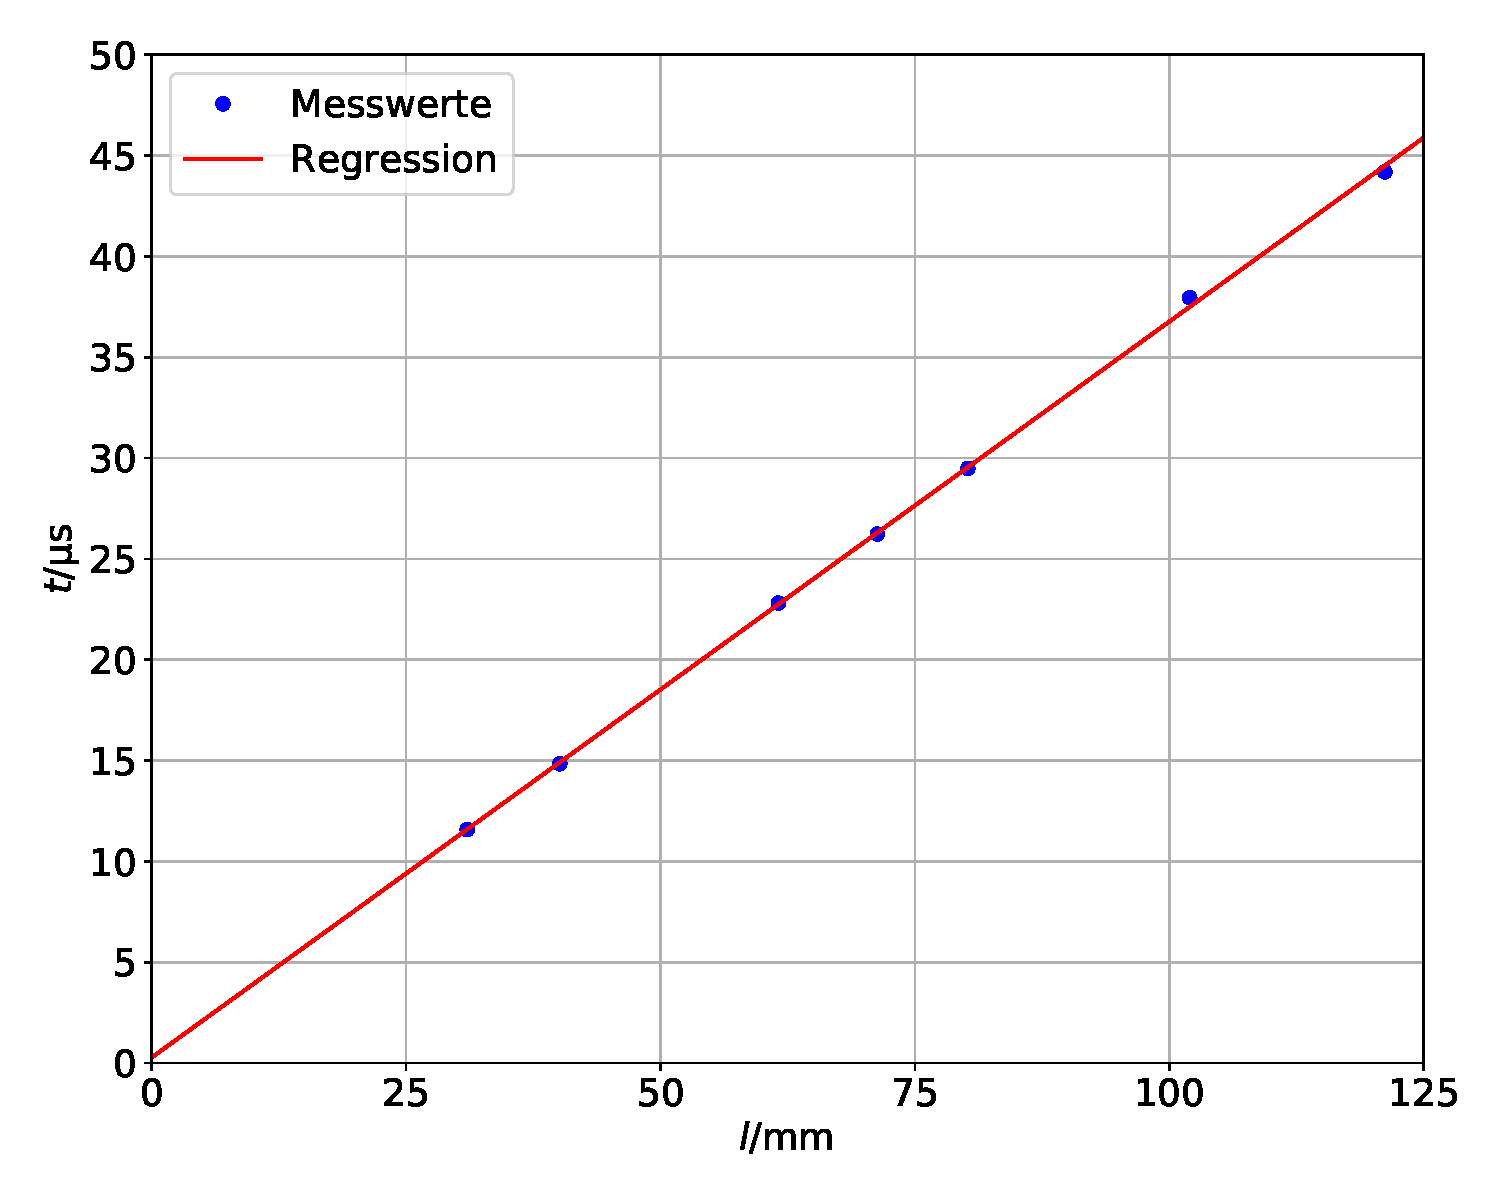
\includegraphics[width=\textwidth]{Imp.pdf}
    \caption{Impuls-Echo-Verfahren}
    \label{abb:1}
  \end{subfigure}
  \begin{subfigure}{0.49\textwidth}
    \centering
    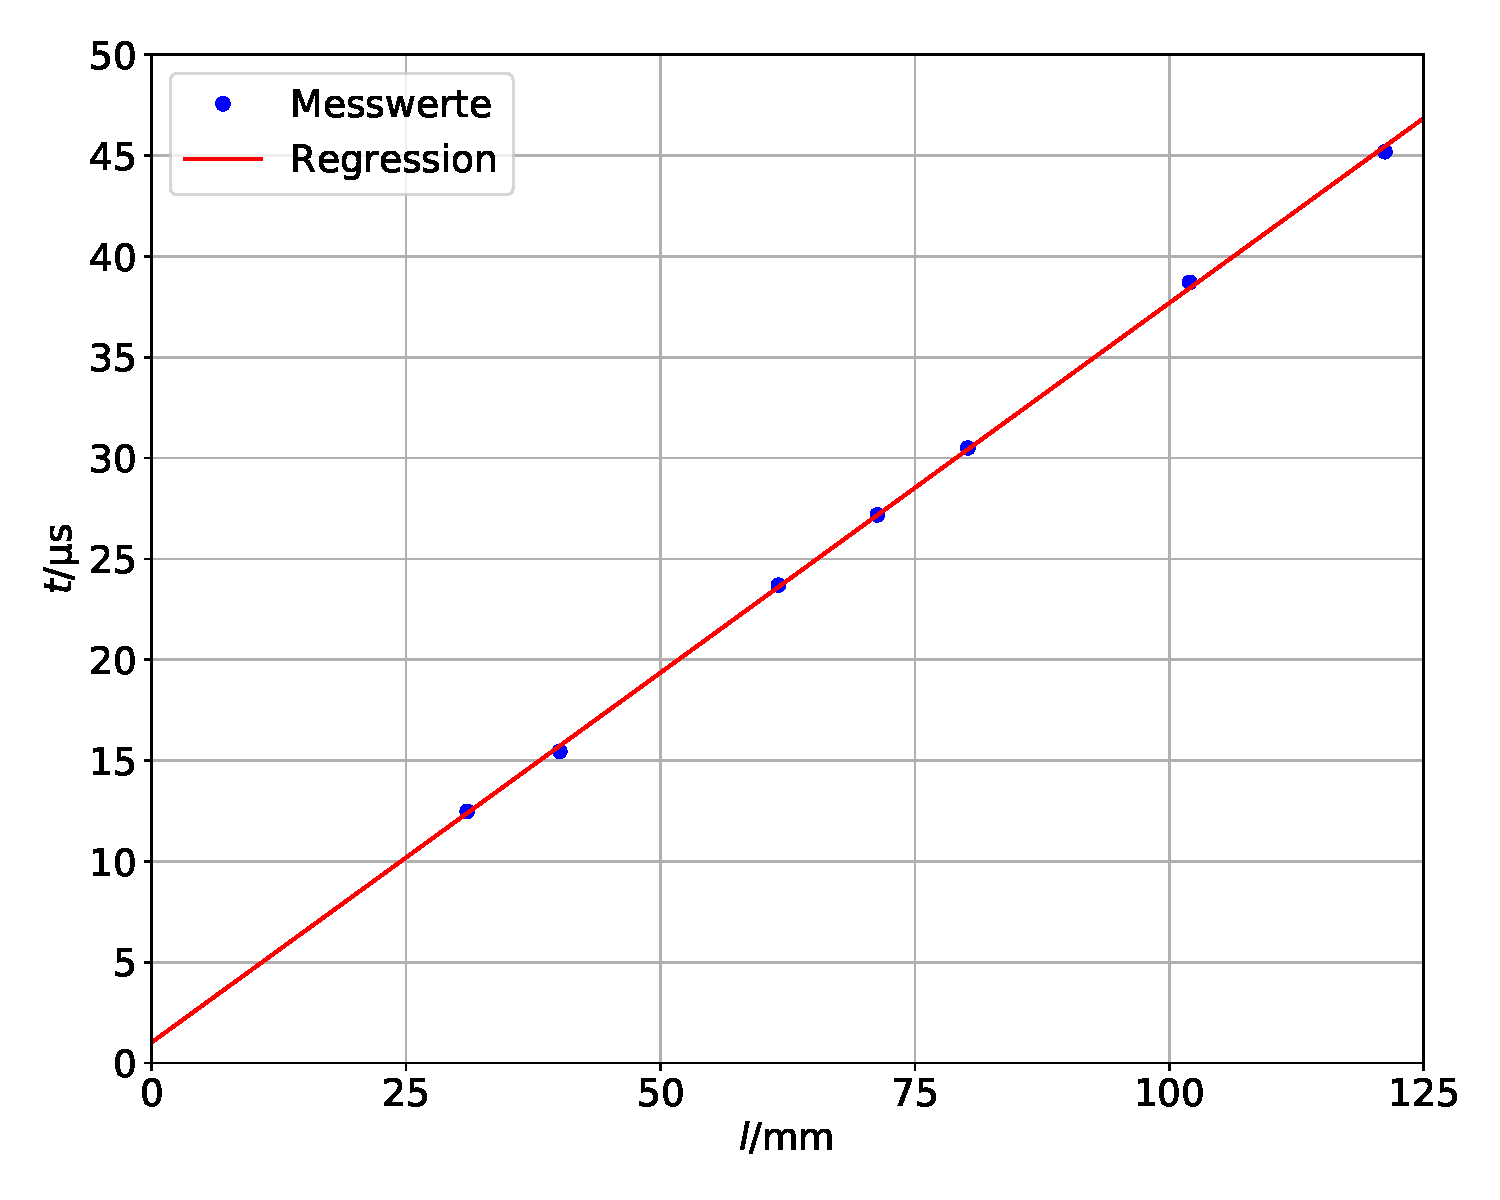
\includegraphics[width=\textwidth]{Dur.pdf}
    \caption{Durchschallverfahren}
    \label{abb:2}
  \end{subfigure}
  \caption{Dargestellt sind die gemessenen Laufzeiten bei beiden Messmethoden mit Regression.
  Insbesondere in \subref{abb:2} erkennt man die Verschiebung des Graphen auf der y-Achse,
  verursacht durch die Schalllaufzeit innerhalb der Sonde, deutlich.}
\end{figure}

\subsection{Betrachtung des Dämpfungsverhaltens von Acryl}
Nun werden die Dämpfungseigenschaften von Acryl betrachtet. Dabei wird die gemessene
Spannungsamplitude des Signals in Abhängigkeit der zurückgelegten Wegstrecke betrachtet.
Zu beachten sind hier drei Dinge:
\begin{enumerate}
  \item Beim Impuls-Echo-Verfahren wird Verfahrensbedingt die dopplete Strecke zurückgelegt.
  \item Manche Amplituden mussten mit Verstärkung gemessen werden. Diese ist in den Tabellen
  \ref{tab:1} und \ref{tab:2} als "TGC"-Wert in \si{\decibel} angegeben. Die Umrechnung in einen
  linearen Faktor geschieht durch:
  \begin{equation}
    G(g) = 10^{ \left( g \cdot \frac{1}{20} \right)}
    \label{eqqA:1}
  \end{equation}
  mit "TGC"-Wert $g$.
  \item Beim Durchschallverfahren wurde eine Empfangsverstärkung von \SI{10}{\decibel}
  zugeschaltet. Diese kann auch nach \ref{eqqA:1} eliminiert werden. Die für beide Verfahren
  genutzte Sendeverstärkung von ebenfalls \SI{10}{\decibel} verbleibt in den Messwerten,
  da sie die gesuchte Größe $\alpha$ sowie die Vergleichbarkeit beider Verfahren nicht beeinflusst.
\end{enumerate}
Die Dämpfung verläuft exponentiell, der Dämpfungskoeffizient $\alpha$ wird daher durch Regression
mit einer Funktion:
\begin{equation}
  U(l) = U_0 * e^{\alpha * l}
\end{equation}
in "phython-scipy" bestimmt. Zu erwähnen ist, dass die für die Zylinder mit Länge
$l=\SI{71.3}{\milli\metre}$ gemessenen Werte nicht genutzt werden können, da dieser
Zylinder aus zwei kürzeren Stücken zusammengesetzt wurde und sich so eine Signalabschwächende
Grenzschicht zwischen den beiden Zylindern bildet. Für das Impuls-Echo-Verfahren ergeben sich:
\begin{align*}
  U_0 &= {0.84(33)}{\volt}\\
  \alpha &= \num{-21(5)}
\end{align*}
und für das Durchschallungsverfahren:
\begin{align*}
  U_0 &= {0.69(18)}{\volt}\\
  \alpha &= \num{-32(11)}
\end{align*}
Die Verläufe mit Regression sind in den Abbildungen \ref{abb:3} und \ref{abb:4} dargestellt.
\begin{figure}
  \centering
  \begin{subfigure}{0.49\textwidth}
    \centering
    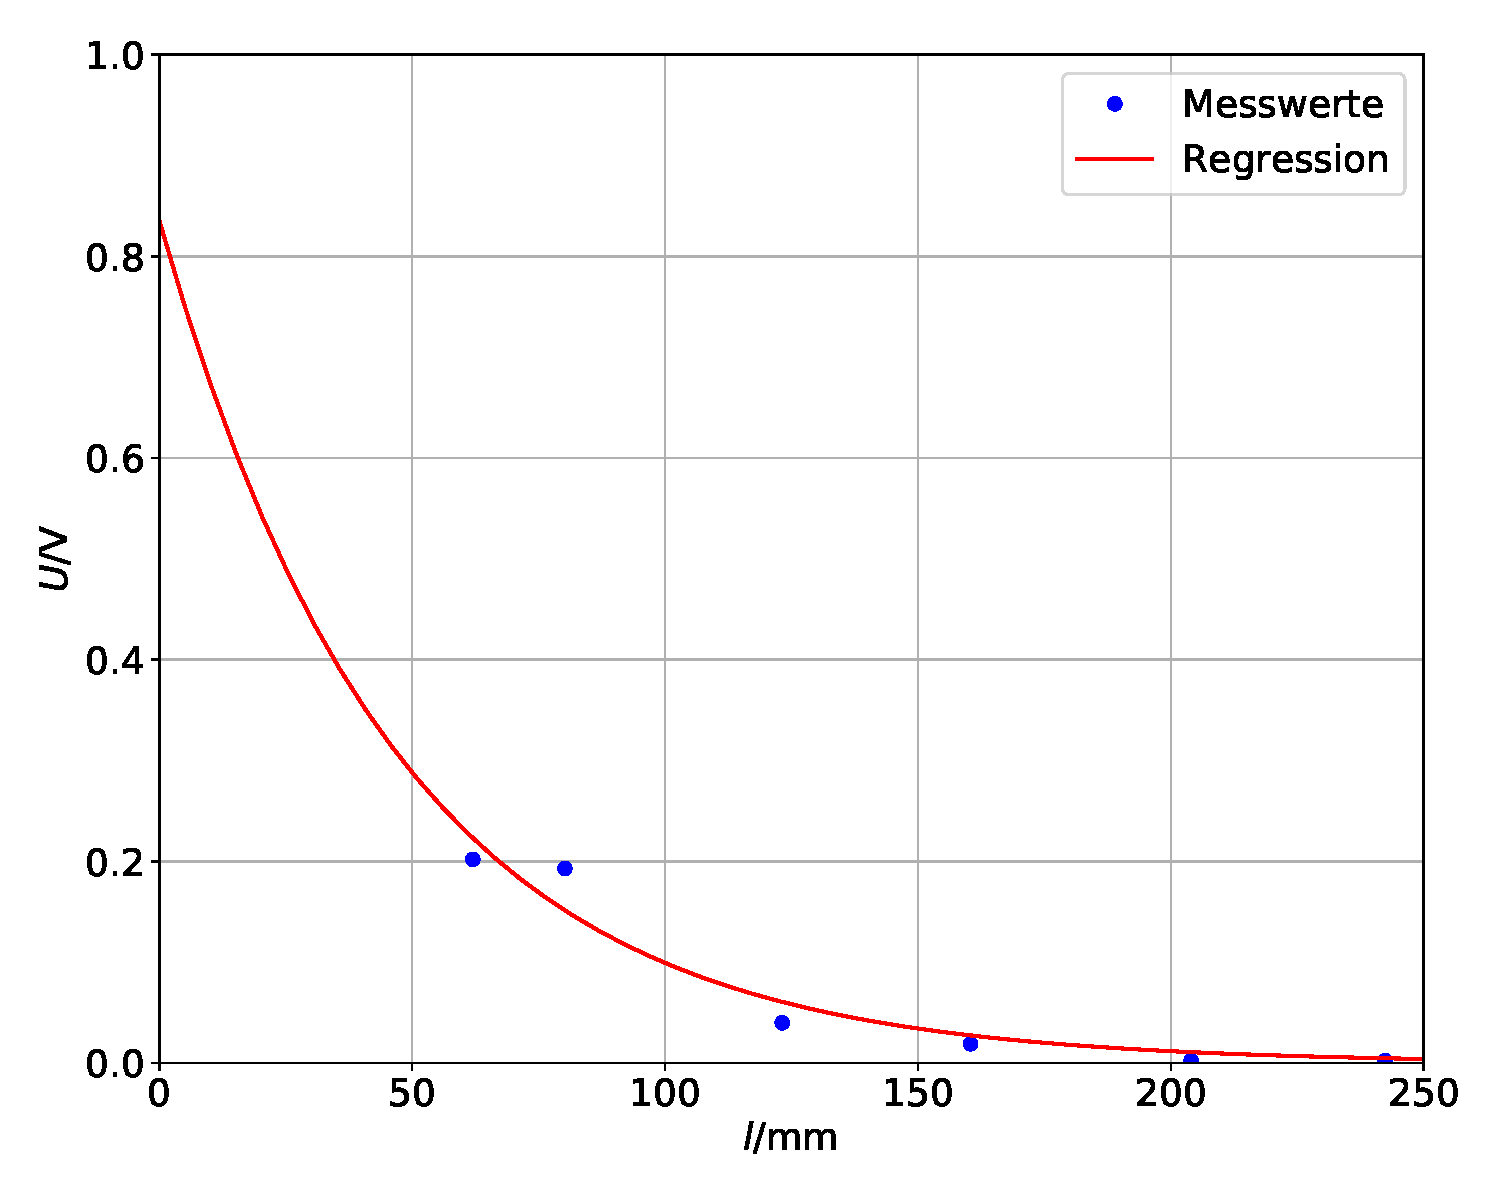
\includegraphics[width=\textwidth]{ImpDump.pdf}
    \caption{Impuls-Echo-Verfahren}
    \label{abb:3}
  \end{subfigure}
  \begin{subfigure}{0.49\textwidth}
    \centering
    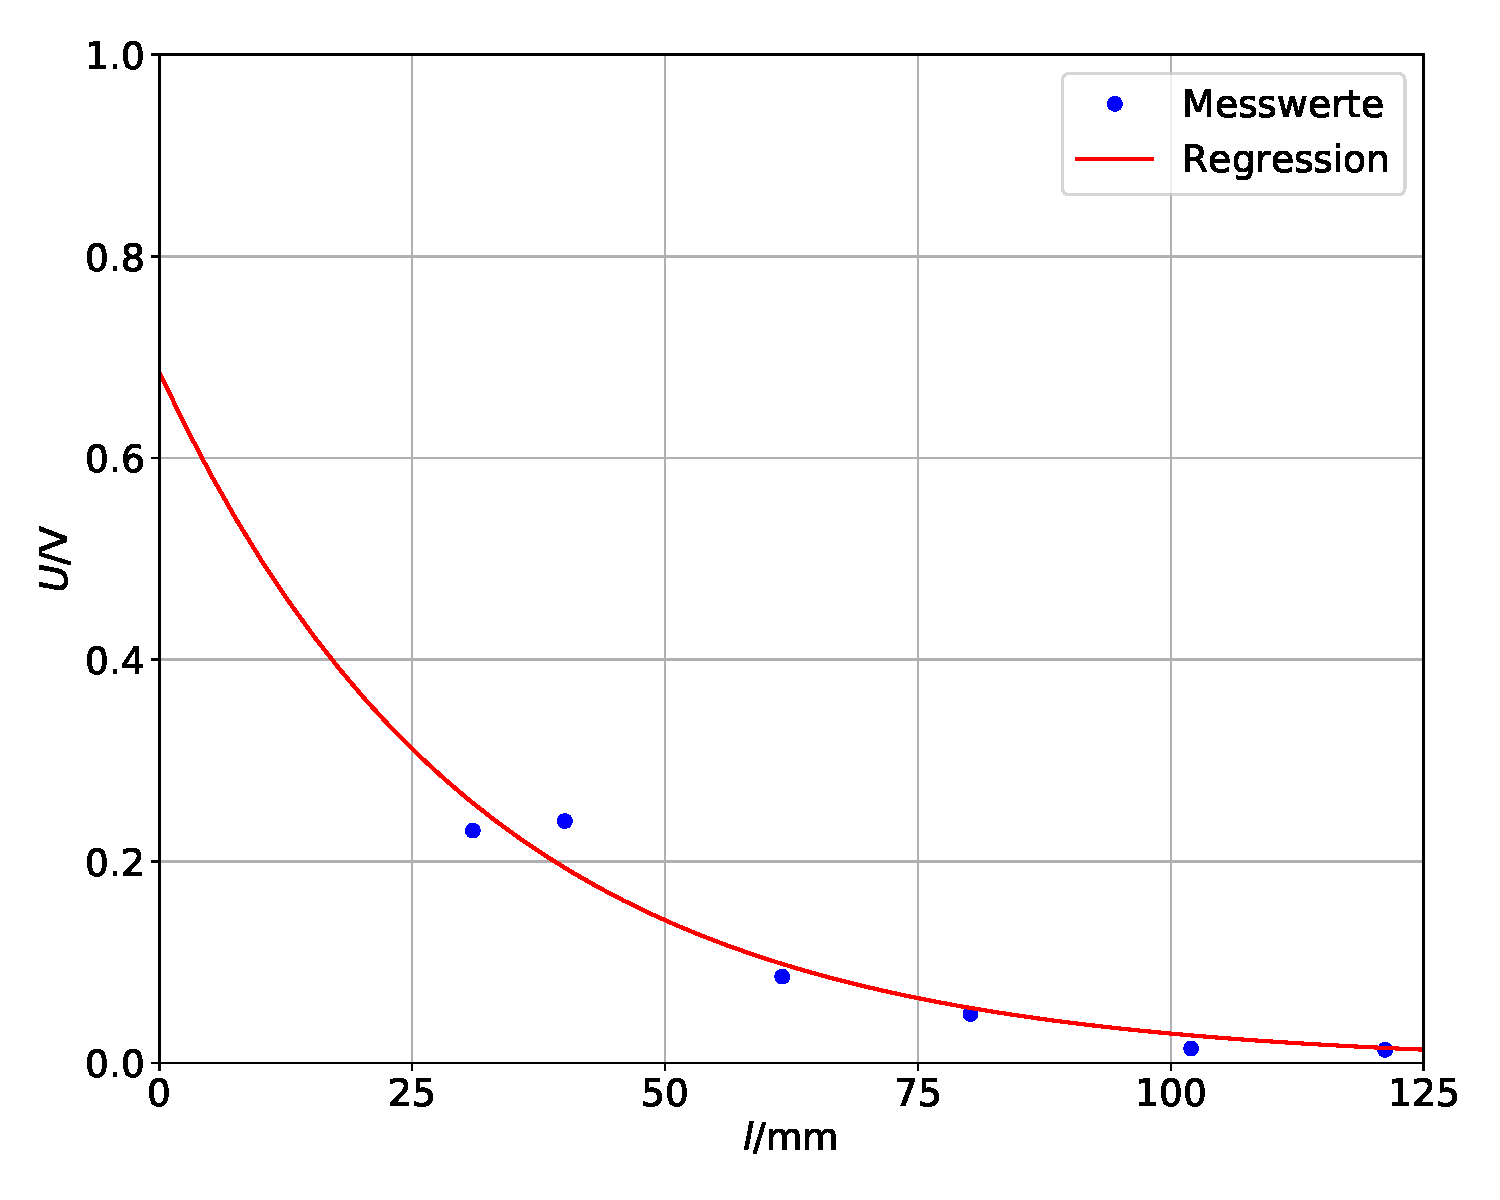
\includegraphics[width=\textwidth]{DurDump.pdf}
    \caption{Durchschallverfahren}
    \label{abb:4}
  \end{subfigure}
  \caption{Dargestellt sind die gemessenen Signalamplituden in Abhängigkeit
  der Signallaufzeit bei beiden Messmethoden mit Regression.}
\end{figure}
\section{Diskussion}
\newpage
\nocite{*}
\printbibliography
